\documentclass[conference]{IEEEtran}
\IEEEoverridecommandlockouts

\usepackage{iftex}
\ifXeTeX % when compiling with XeTeX (e.g. tectonic), still use IEEE's Times font
  \usepackage{fontspec}
  \setmainfont{texgyretermes}[Extension=.otf, UprightFont=*-regular, BoldFont=*-bold,
    ItalicFont=*-italic, BoldItalicFont=*-bolditalic]
\fi
\usepackage{cite}
\usepackage{amsmath,amssymb}
\usepackage{graphicx}
\usepackage{booktabs}
\usepackage{multirow}
\usepackage{xcolor}
\usepackage{url}
\usepackage[hidelinks]{hyperref}

\graphicspath{{figures/}}
% Float settings so that figures are placed close to the text
\renewcommand{\topfraction}{0.9}
\renewcommand{\dbltopfraction}{0.9}
\renewcommand{\textfraction}{0.07}
\renewcommand{\floatpagefraction}{0.8}
\renewcommand{\dblfloatpagefraction}{0.8}

\begin{document}

\title{Beyond FLOPs: An Experimental Time--Space--Energy--Performance Analysis of Deep Image Classifiers on CIFAR-10}

% ---- Author information: fill in the details of all group members ----
% AISCI 2027 uses double-blind review: for a real conference submission set
% \blindtrue below to hide the names (the course version keeps them).
\newif\ifblind
\blindfalse
\ifblind
\author{\IEEEauthorblockN{Anonymous Authors}\IEEEauthorblockA{\textit{Under double-blind review}}}
\else
\author{
\IEEEauthorblockN{Muhammed Enes Akça}
\IEEEauthorblockA{\textit{Department of Computer Engineering} \\
\textit{Istanbul Health and Technology}\\
\textit{University}\\
Istanbul, Turkey \\
menes.akca@hotmail.com}
\and
\IEEEauthorblockN{İdris Salih Yıldırım}
\IEEEauthorblockA{\textit{Department of Computer Engineering} \\
\textit{Istanbul Health and Technology}\\
\textit{University}\\
Istanbul, Turkey \\
idrisalih27@gmail.com}
\and
\IEEEauthorblockN{Yağmur Öztürk}
\IEEEauthorblockA{\textit{Department of Computer Engineering} \\
\textit{Istanbul Health and Technology}\\
\textit{University}\\
Istanbul, Turkey \\
ozturkyagmur521@gmail.com}
}
\fi

\maketitle

\begin{abstract}
Deep learning models are usually compared by accuracy and by hardware-independent cost proxies such as parameter count and floating-point operations (FLOPs). We test how well these proxies predict the real cost of training and inference. Five image classifiers of increasing complexity (an MLP, two plain CNNs, MobileNetV2 and ResNet-18) are trained on CIFAR-10 with one shared recipe on a single consumer laptop GPU (RTX~4060). We vary the training-set size (10--100\%) and repeat every configuration with five seeds, giving 100 runs. Each run records accuracy, macro precision, recall and F1, training and inference time, peak RAM and VRAM, and GPU energy from the hardware counter, cross-checked with power sampling and CodeCarbon. Training time and energy grow linearly with data size (fitted exponent $0.96$--$1.01$, $R^2\geq0.99$) while GPU memory stays constant, as the theory predicts. Across architectures, however, FLOPs are a poor predictor. MobileNetV2 needs $6.3\times$ fewer FLOPs than ResNet-18 yet trains $1.4\times$ slower, uses $1.47\times$ more energy and $2.6\times$ more training VRAM. It sustains only 1.3 vs.\ 11.5~TFLOP/s on the GPU. A medium-sized CNN reaches 89.4\% accuracy with $7.8\times$ less energy than ResNet-18 (92.9\%) and dominates the accuracy--energy Pareto front. Hardware utilisation, not operation count, drives the measured cost.
\end{abstract}

\begin{IEEEkeywords}
algorithm analysis, computational complexity, energy efficiency, green AI, convolutional neural networks, benchmarking, CIFAR-10
\end{IEEEkeywords}

% =====================================================================
\section{Introduction}
% =====================================================================
Classic algorithm analysis describes cost with asymptotic bounds on time and space. Deep learning models are compared the same way, with hardware-independent proxies: the number of trainable parameters stands in for memory, and the number of floating-point operations (FLOPs) per input stands in for time. These proxies are convenient, but a model does not run on an abstract machine. It runs on a processor with finite memory bandwidth, kernel-launch overheads and a power budget. The question is therefore not only \emph{how many} operations a model performs but \emph{how efficiently} the hardware can perform them~\cite{williams2009roofline,sze2017efficient}.

The energy cost of deep learning has also become a concern in its own right. Training large models can have a measurable carbon footprint~\cite{strubell2019energy,patterson2021carbon}, and the ``Green AI'' agenda argues that efficiency should be reported next to accuracy~\cite{schwartz2020green,henderson2020systematic}. Energy is linked to time through $E = P_{\mathrm{avg}}\cdot T$, but the average power $P_{\mathrm{avg}}$ itself depends on the workload. A shorter run is therefore not automatically a cheaper one.

This paper studies these questions experimentally. We train five models of increasing complexity on CIFAR-10~\cite{krizhevsky2009cifar} under identical conditions and measure four cost dimensions together: performance, time, space and energy. Our contributions are: (i) a controlled benchmark of five architectures, from a 20\,k-parameter CNN to an 11\,M-parameter ResNet-18, over 4 training-set sizes $\times$ 5 seeds (100 runs), with training and inference measured separately; (ii) a validated energy-measurement protocol based on the GPU's hardware energy counter, compared with 10\,Hz power sampling and CodeCarbon~\cite{codecarbon}; (iii) a direct comparison of theoretical cost (FLOPs, parameters, asymptotic complexity) with measured time, memory and energy, showing that data-size scaling follows the theory while FLOP-based predictions across architectures fail; and (iv) an accuracy--energy trade-off analysis that identifies Pareto-optimal models and quantifies diminishing returns.

% =====================================================================
\section{Related Work}
% =====================================================================
\textbf{Efficient architectures.} ResNet~\cite{he2016resnet} introduced residual connections that make deep CNNs trainable. MobileNets~\cite{howard2017mobilenets} and MobileNetV2~\cite{sandler2018mobilenetv2} use depthwise-separable convolutions and inverted residual blocks to cut FLOPs and parameters, mainly for mobile CPUs. Ma \emph{et al.}~\cite{ma2018shufflenetv2} showed that FLOPs are an \emph{indirect} metric. Memory access cost and the degree of parallelism also determine speed, and models with similar FLOPs can differ greatly in latency. Canziani \emph{et al.}~\cite{canziani2016analysis} reported accuracy, inference time, memory and power for ImageNet models on an embedded GPU and found that power draw is roughly independent of model size.

\textbf{Performance models.} The roofline model~\cite{williams2009roofline} explains attainable throughput through arithmetic intensity, the number of operations per byte moved. Operations with low intensity, such as depthwise convolutions, are memory-bound. Sze \emph{et al.}~\cite{sze2017efficient} survey why data movement, rather than arithmetic, dominates the energy cost of DNN accelerators.

\textbf{Energy and carbon accounting.} Strubell \emph{et al.}~\cite{strubell2019energy} estimated the energy and carbon of NLP model training; systematic reporting tools and estimation methods were proposed and reviewed in~\cite{henderson2020systematic,lacoste2019quantifying,garciamartin2019estimation}, and cloud training and inference-energy trends were studied in~\cite{dodge2022measuring,desislavov2023trends}. Most of these studies rely on software estimates or on large data-centre hardware.

\textbf{Scaling.} Empirical scaling studies~\cite{hestness2017scaling,kaplan2020scaling} show that error falls as a power law in data and compute. Our data-size sweep is a small-scale view of the same diminishing-returns behaviour.

We complement them with a controlled, repeated ($n{=}5$) benchmark on consumer hardware that separates training from inference and reads energy directly from the hardware counter.

% =====================================================================
\section{Theoretical Background and Complexity Analysis}
% =====================================================================
\subsection{Per-layer cost}
Let $F$ be the FLOPs of one forward pass; one multiply--accumulate counts as two FLOPs.
\begin{itemize}
  \item \textbf{Fully connected layer} ($d_{\mathrm{in}}\!\to\!d_{\mathrm{out}}$): $d_{\mathrm{in}}d_{\mathrm{out}}$ parameters and $2d_{\mathrm{in}}d_{\mathrm{out}}$ FLOPs. For our MLP (3072--512--256--10) this gives $1.71$\,M parameters and $3.4$\,MFLOPs per image. Here the parameter count and the compute are of the same order.
  \item \textbf{Standard convolution} ($K\times K$, $C_{\mathrm{in}}\!\to\!C_{\mathrm{out}}$, output $H\times W$): $K^2C_{\mathrm{in}}C_{\mathrm{out}}$ parameters and
  \begin{equation}
     F_{\mathrm{conv}} = 2\,HW K^2 C_{\mathrm{in}} C_{\mathrm{out}}
  \end{equation}
  FLOPs. Weights are reused at every spatial position, so FLOPs grow with $HW$ while the number of parameters does not. This is why our SmallCNN has $85\times$ fewer parameters than the MLP but $3.3\times$ more FLOPs.
  \item \textbf{Depthwise-separable convolution}~\cite{howard2017mobilenets}: a per-channel $K\times K$ convolution followed by a $1\times1$ convolution. It costs $2HW C(K^2 + C_{\mathrm{out}})$ FLOPs, a reduction by a factor of $1/C_{\mathrm{out}} + 1/K^2$ compared with a standard convolution. Its arithmetic intensity, however, is low. Each depthwise output reads $K^2$ inputs but performs only $K^2$ MACs, so the operation tends to be memory-bound~\cite{williams2009roofline,ma2018shufflenetv2}.
\end{itemize}

\subsection{Training and inference time}
A training epoch processes $n$ images in $\lceil n/B\rceil$ mini-batches. Backpropagation costs about twice the forward pass, so the total training work is approximately
\begin{equation}
   W_{\mathrm{train}}(n) \approx 3\,F\,n\,E_p ,
   \label{eq:work}
\end{equation}
where $E_p$ is the number of epochs. The training time is $T_{\mathrm{train}} = W_{\mathrm{train}}/R$, where $R$ is the achieved throughput in FLOP/s. For a fixed model $T_{\mathrm{train}}(n)=\Theta(n)$. Comparing \emph{different} models by $F$ alone implicitly assumes that $R$ is the same for all of them. Our experiments test this assumption. Inference costs $\Theta(F)$ per image, so the time for $m$ test images is $\Theta(mF)/R$.

\subsection{Memory}
Training with SGD and momentum stores the weights, the gradients and one momentum buffer: $3P$ values for $P$ parameters. The forward activations must also be kept for the backward pass:
\begin{equation}
   M_{\mathrm{train}} \approx 3P\cdot b + B\sum_{\ell} a_\ell \cdot b',
\end{equation}
where $a_\ell$ is the activation size of layer $\ell$ and $b, b'$ are bytes per value. Inference needs only $P$ and the largest live activations. Architectures with many wide intermediate tensors, such as the expanded layers of inverted residual blocks~\cite{sandler2018mobilenetv2}, can therefore need more training memory than models with many more parameters.

\subsection{Energy}
The energy is the integral of power over time:
\begin{equation}
   E = \int_0^{T} P(t)\,dt = P_{\mathrm{avg}}\cdot T.
\end{equation}
We split it into an idle (static) part and a dynamic part, $E_{\mathrm{dyn}} = E - P_{\mathrm{idle}}\,T$. Because $P_{\mathrm{avg}}$ depends on how intensively the hardware is used, two runs of equal length can consume different amounts of energy.

% =====================================================================
\section{Methodology and Experimental Setup}
% =====================================================================
\subsection{Dataset and subsets}
CIFAR-10~\cite{krizhevsky2009cifar} contains 50{,}000 training and 10{,}000 test RGB images ($32\times32$) in 10 balanced classes. There is no separate validation split. The pilot that fixed the recipe monitored test accuracy, so to limit selection bias the recipe is shared by all models and never tuned per model, and every reported metric is taken after the final epoch, not at the best one. Images are normalised with the training-set mean and standard deviation. To study data scaling we draw \emph{nested, stratified} training subsets of 10, 25, 50 and 100\% (5k, 12.5k, 25k, 50k images) with a fixed seed. Every subset keeps the class balance and is contained in the next larger one.

\subsection{Models}
Table~\ref{tab:main} lists the parameters and FLOPs of the five models: an \textbf{MLP} (3072--512--256--10 with batch normalisation~\cite{ioffe2015batchnorm} and dropout 0.3); \textbf{SmallCNN}, two $3\times3$ conv--BN--ReLU layers (32 and 64 filters), each followed by $2\times2$ max-pooling, then global average pooling and a linear classifier (20\,k parameters); \textbf{MediumCNN}, a VGG-style network of three blocks with two $3\times3$ conv--BN--ReLU layers each (32/64/128 filters), max-pooling after each block, global average pooling and a linear classifier (0.29\,M parameters); \textbf{MobileNetV2}~\cite{sandler2018mobilenetv2}, the standard inverted-residual network with expansion factor 6, adapted to $32\times32$ inputs by using stride 1 in the first convolution and the second stage; and \textbf{ResNet-18}~\cite{he2016resnet}, the CIFAR variant ($3\times3$ stem, no initial max-pool). FLOPs were counted with PyTorch's \texttt{FlopCounterMode} for a single $32\times32$ image.

\subsection{Training recipe}
All models share one recipe so that the comparison is fair. We use 30 epochs, batch size 128, SGD with Nesterov momentum 0.9, learning rate 0.05, weight decay $5\cdot10^{-4}$, and a cosine learning-rate schedule~\cite{loshchilov2017sgdr} stepped every batch. Augmentation consists of a random horizontal flip and a random 4-pixel-padded crop, both applied on the GPU. All runs use bfloat16 mixed precision~\cite{micikevicius2018mixed}. The recipe was fixed during a pilot study, before any measurement, and is not tuned per model.

\subsection{Hardware and software}
All runs used one laptop: an HP Victus~16 with an AMD Ryzen~7 7840HS (8 cores/16 threads), 32\,GB RAM, and an NVIDIA GeForce RTX~4060 Laptop GPU (8\,GB VRAM; driver 621.24; power limit 113\,W in the vendor's ``Performance'' mode). The operating system was Windows~11. The software stack was Python~3.12.10, PyTorch~2.11.0 with CUDA~12.8 and cuDNN~9.19~\cite{paszke2019pytorch}, scikit-learn~1.9.1 and CodeCarbon~3.3.2. During the measurement session the fan was set to maximum and an external cooling pad was used, all other applications were closed, and the machine was on mains power.

\subsection{Measurement protocol}
\textbf{Experiment design.} The 5 models $\times$ 4 data sizes $\times$ 5 seeds (0--4) give 100 runs in total. Seeds form the outer loop. Within each seed the 20 runs are executed in a fixed random order, so slow drifts such as heating are not confounded with a model. Before each run the script waits until the GPU is below 60\,$^\circ$C and then records the idle GPU power for 5\,s.

\textbf{Warm-up.} cuDNN autotuning and lazy kernel loading made the first epoch more than $10\times$ slower than the following ones in a pilot (18.6\,s vs.\ 1.6\,s). Each run therefore starts with an unmeasured warm-up that trains a throw-away copy of the architecture on random data, using every batch shape that will occur.

\textbf{Time.} Wall-clock time is taken with \texttt{perf\_counter}, with \texttt{cuda.synchronize()} before each reading. Training time covers all 30 epochs. Inference is measured in two ways. \emph{Throughput}: the full test set is processed in batches of 512, repeated until at least 10\,s and 3 passes have elapsed. \emph{Latency}: 300 single images (batch size 1, after 30 warm-up images) are timed, including the host-to-device copy and the transfer of the result back to the CPU.

\textbf{Space.} Peak VRAM is the peak memory allocated by PyTorch; peak RAM is the peak resident set size of the process, sampled at 10\,Hz. \textbf{Energy.} The primary measure is the GPU's cumulative hardware energy counter, read through NVML~\cite{nvml}. As a cross-check, power is sampled at 10\,Hz and integrated with the trapezoidal rule. CodeCarbon~\cite{codecarbon} additionally estimates GPU, CPU and RAM energy and CO$_2$ (Turkish grid intensity). Because the AMD CPU exposes no RAPL interface to user space, CPU energy is \emph{estimated} by CodeCarbon rather than measured, and we report it only as such.

\textbf{Performance and statistics.} We report accuracy and macro-averaged precision, recall and F1 on the full 10{,}000-image test set. All values are means $\pm$ standard deviations over the 5 seeds; scaling exponents are least-squares fits in log--log space.

% =====================================================================
\section{Experimental Results and Discussion}
% =====================================================================
All 100 runs completed without error in 3\,h\,38\,min. Measurement stability was high. The five repetitions of ResNet-18 on the full data, spread across the session, took 432--437\,s at a mean GPU clock of 2505--2512\,MHz, and the maximum GPU temperature over all runs was 73\,$^\circ$C. Seed-to-seed coefficients of variation of training time and energy were below 0.5\% for the two large models.

\begin{table*}[t]
\centering
\caption{Main results on the full training set (50k images). Mean $\pm$ std over 5 seeds. Energy is GPU energy from the hardware counter. Throughput and inference energy are measured at batch 512, latency (median) at batch 1.}
\label{tab:main}
\setlength{\tabcolsep}{3.5pt}
\begin{tabular}{lrrcccrrrcr}
\toprule
 & Params & MFLOPs & Accuracy & Train time & Train energy & \multicolumn{2}{c}{Peak VRAM (MB)} & Throughput & Infer energy & Latency \\
Model & (M) & /img & (\%) & (s) & (kJ) & train & infer & (img/s) & (mJ/img) & (ms) \\
\midrule
MLP         & 1.71  & 3.4    & 57.18$\pm$0.32 & 35.4$\pm$0.8  & 1.22$\pm$0.04  & 58   & 43  & 515{,}762 & 0.08$\pm$0.00  & 0.42 \\
SmallCNN    & 0.02  & 11.2   & 69.03$\pm$0.33 & 35.8$\pm$1.0  & 2.16$\pm$0.04  & 63   & 95  & 203{,}230 & 0.39$\pm$0.01  & 0.51 \\
MediumCNN   & 0.29  & 77.3   & 89.43$\pm$0.08 & 62.7$\pm$3.0  & 4.66$\pm$0.12  & 104  & 154 & 90{,}687  & 0.96$\pm$0.01  & 1.15 \\
MobileNetV2 & 2.24  & 176.0  & 91.76$\pm$0.15 & 606.2$\pm$1.6 & 53.75$\pm$0.09 & 1227 & 354 & 8{,}276   & 10.38$\pm$0.06 & 6.62 \\
ResNet-18   & 11.17 & 1110.8 & \textbf{92.87$\pm$0.35} & 434.4$\pm$1.9 & 36.56$\pm$0.12 & 476  & 495 & 10{,}532  & 8.04$\pm$0.07  & 3.30 \\
\bottomrule
\end{tabular}
\end{table*}

\subsection{Performance}
Table~\ref{tab:metrics} lists all four classification metrics on the full training set. Accuracy rises from 57.2\% (MLP) to 92.9\% (ResNet-18), and the seed-to-seed standard deviation is at most 0.37 points for every metric. CIFAR-10 is class-balanced, so the four metrics agree to within 0.5 points; macro recall even equals accuracy exactly, because every test class has the same number of images. The MLP ignores spatial structure, which caps its accuracy far below the convolutional models. Even the 20\,k-parameter SmallCNN outperforms it by 12 points.

\begin{table}[t]
\centering
\caption{Classification performance on the full training set (\%, macro-averaged over the 10 classes; mean $\pm$ std over 5 seeds).}
\label{tab:metrics}
\setlength{\tabcolsep}{3pt}
\begin{tabular}{lcccc}
\toprule
Model & Accuracy & Precision & Recall & F1 \\
\midrule
MLP         & 57.18$\pm$0.32 & 56.81$\pm$0.30 & 57.18$\pm$0.32 & 56.68$\pm$0.34 \\
SmallCNN    & 69.03$\pm$0.33 & 68.93$\pm$0.35 & 69.03$\pm$0.33 & 68.86$\pm$0.37 \\
MediumCNN   & 89.43$\pm$0.08 & 89.42$\pm$0.10 & 89.43$\pm$0.08 & 89.41$\pm$0.08 \\
MobileNetV2 & 91.76$\pm$0.15 & 91.75$\pm$0.14 & 91.76$\pm$0.15 & 91.74$\pm$0.14 \\
ResNet-18   & \textbf{92.87$\pm$0.35} & \textbf{92.88$\pm$0.34} & \textbf{92.87$\pm$0.35} & \textbf{92.87$\pm$0.34} \\
\bottomrule
\end{tabular}
\end{table}

\subsection{Scaling with data size: theory confirmed}
Fig.~\ref{fig:scaling} shows all four cost dimensions against the training-set size $n$.

\emph{Time} (Fig.~\ref{fig:scaling}(a)). Equation~\eqref{eq:work} predicts $T\propto n$. The fitted log--log exponents are $k=0.990$--$0.999$ for all five models ($R^2\geq0.998$). The slightly sub-linear exponents of the smallest models come from fixed per-epoch overheads that are not amortised for $n=5$k.

\emph{Energy} (Fig.~\ref{fig:scaling}(b)). Energy grows linearly as well ($k=0.96$--$1.01$). Since $E=P_{\mathrm{avg}}\cdot T$, this means that the average power of a model does not depend on $n$; only the running time does.

\emph{Space} (Fig.~\ref{fig:scaling}(c)). Peak training VRAM is constant in $n$: it changes by less than 1\% between 5k and 50k images. The data is streamed to the GPU in mini-batches of fixed size, so GPU memory depends on the model and the batch size but not on the dataset size; the GPU space complexity is $O(1)$ in $n$. Peak host RAM did not grow with $n$ either (median 3.5\,GB; only the first runs of the session, before all libraries were loaded, needed 2.7--3.1\,GB): it is dominated by the framework and the in-memory dataset, which is loaded once regardless of the subset.

\emph{Performance} (Fig.~\ref{fig:scaling}(d)). Accuracy grows sub-linearly with $n$, the expected diminishing return~\cite{hestness2017scaling}. The ranking of the models also depends on $n$. With 5k images MediumCNN (72.4\%) clearly beats both ResNet-18 ($63.3\pm2.0$\%) and MobileNetV2 (66.6\%). The large models only overtake it once 25k or more images are available. Their higher capacity needs more data to pay off, and with little data they are also less stable across seeds (std 2.0 vs.\ 0.4).

The asymptotic analysis is thus an excellent \emph{within-model} predictor: time and energy are $\Theta(n)$ and GPU memory is $O(1)$ in $n$, exactly as derived in Section~III.

\begin{figure*}[t]
\centering
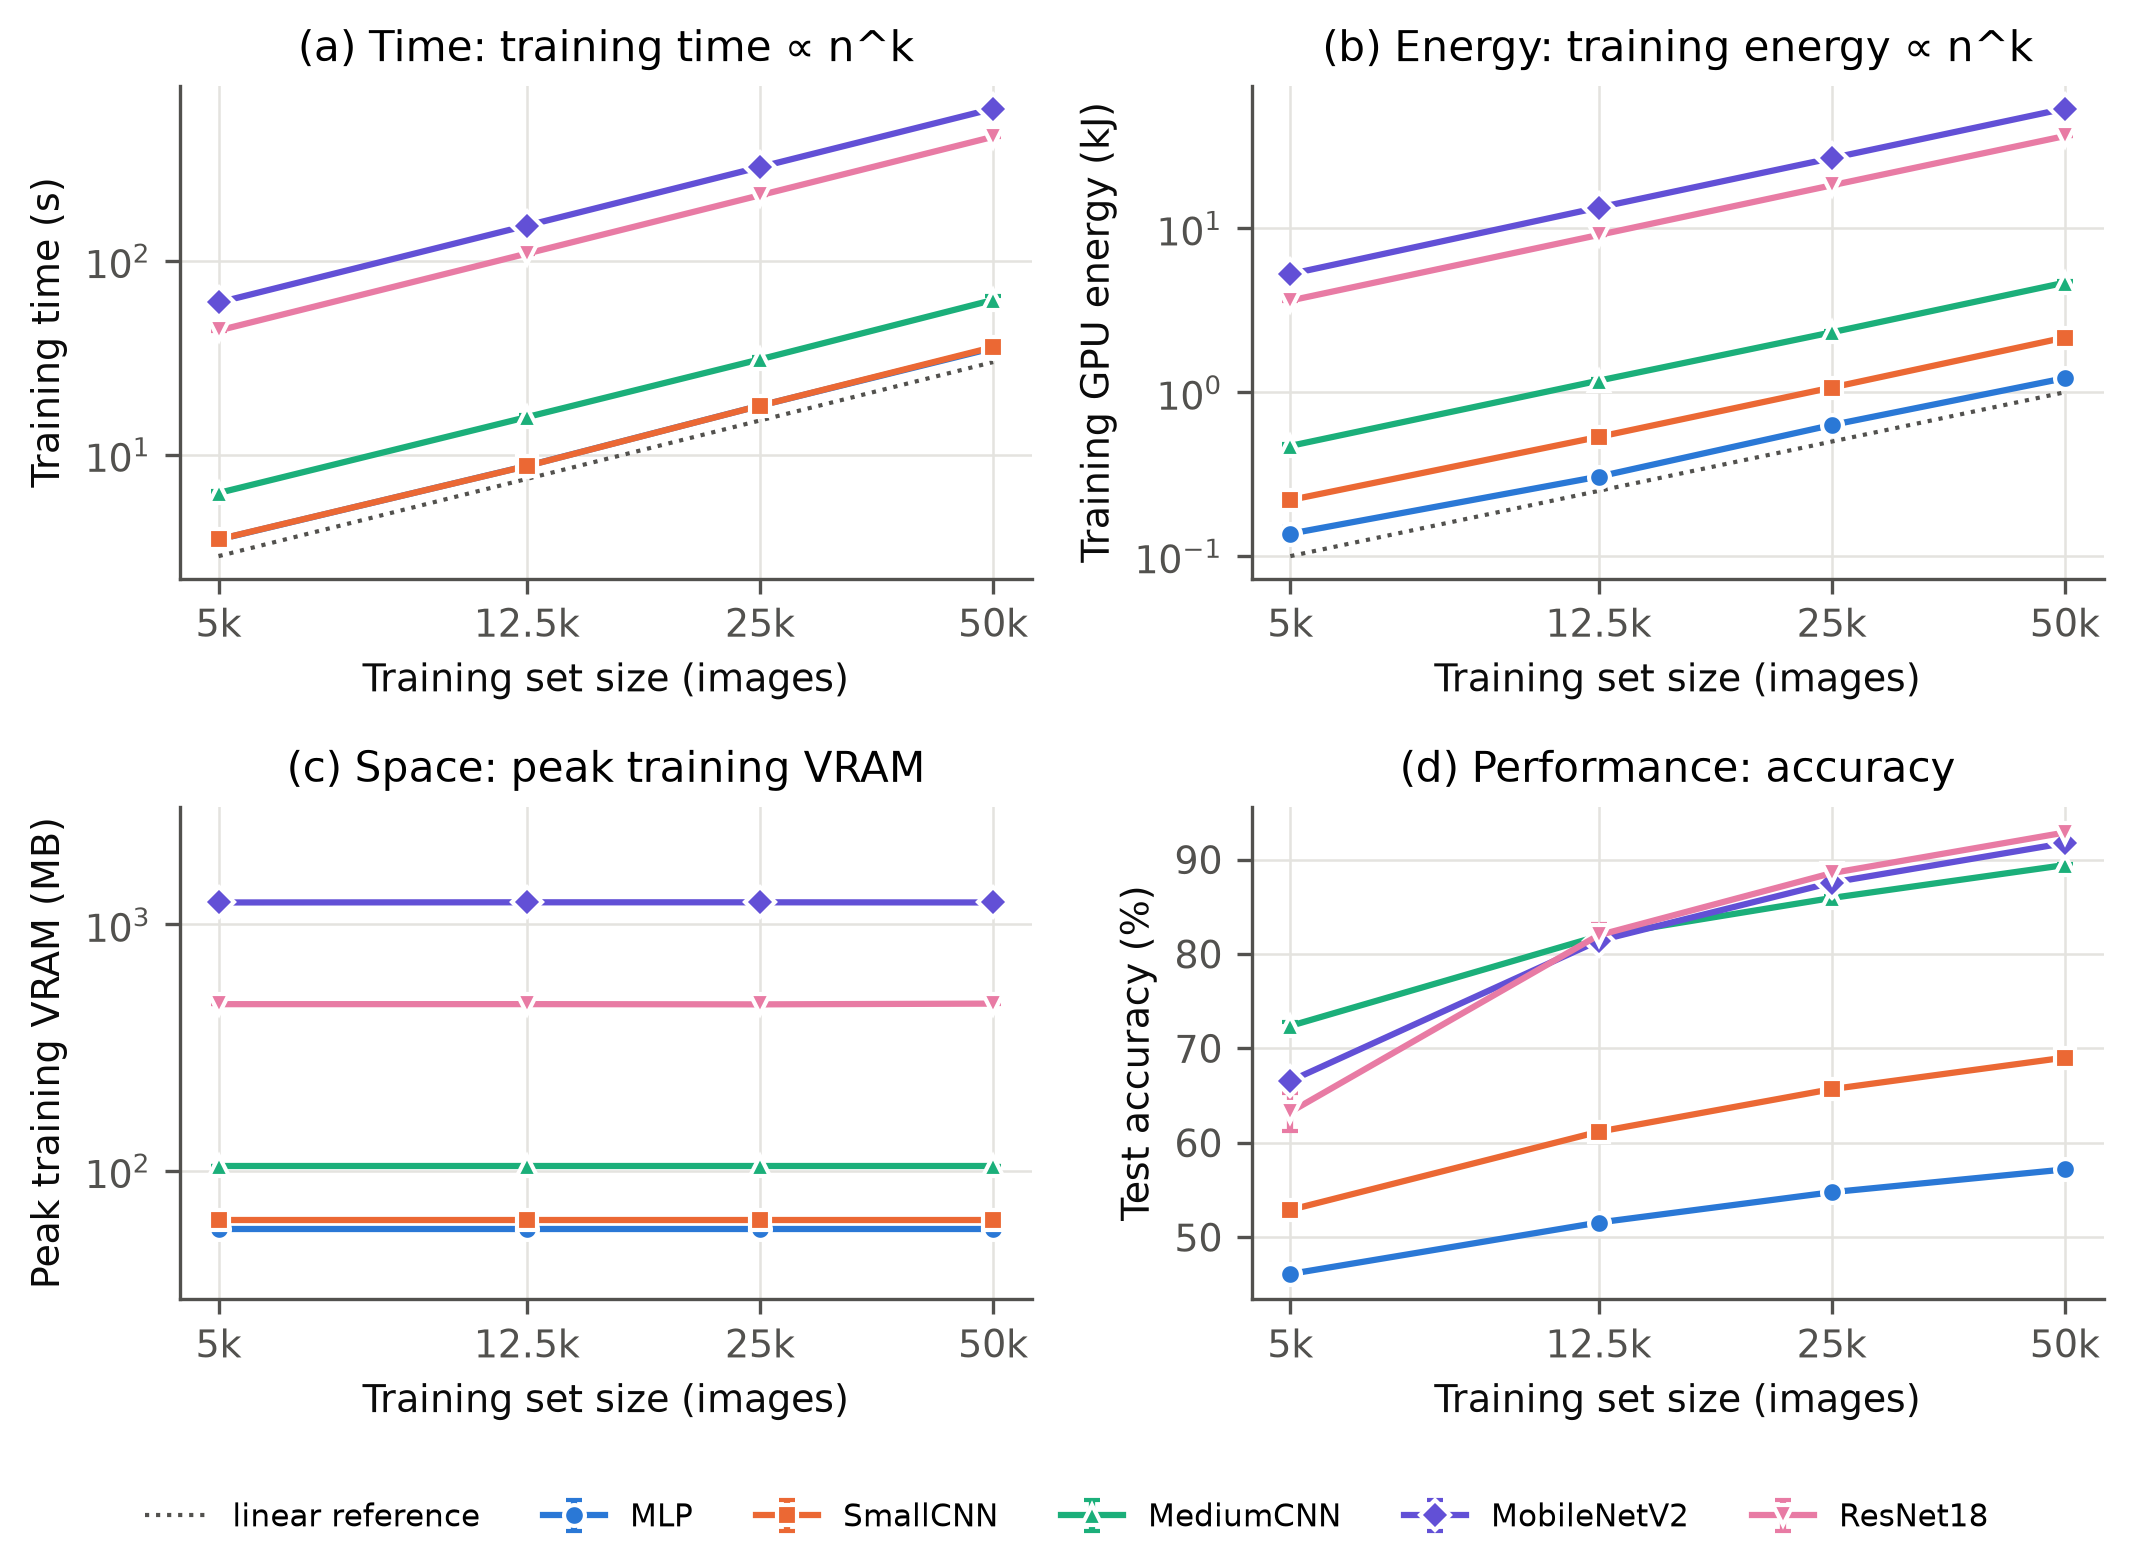
\includegraphics[width=0.6\textwidth]{fig2_scaling.png}
\caption{The four cost dimensions vs.\ training-set size $n$: (a) training time and (b) training GPU energy (log--log; fitted exponents of $T, E\propto n^k$ are $k=0.99$--$1.00$ for time and $0.96$--$1.01$ for energy; the dotted line shows linear scaling), (c) peak training VRAM, (d) test accuracy. Error bars show $\pm1$ std over 5 seeds.}
\label{fig:scaling}
\end{figure*}

\subsection{Theory vs.\ measurement across architectures}
If time were proportional to FLOPs, all models in Fig.~\ref{fig:theory}(a) would lie on the dashed line. The rank correlation between FLOPs and training time is high (Spearman $\rho=0.90$), but the magnitudes are far off. Relative to ResNet-18, \textbf{MobileNetV2} needs 0.16$\times$ the FLOPs but 1.40$\times$ the training time, 1.47$\times$ the training energy and 1.27$\times$ the inference time per image, while \textbf{MLP} and \textbf{SmallCNN} need 0.3\% and 1.0\% of the FLOPs but 8\% of the training time.
The explanation is the achieved throughput $R$ in Eq.~\eqref{eq:work} (Fig.~\ref{fig:theory}(b)). ResNet-18 sustains 11.5~TFLOP/s in training because its dense $3\times3$ convolutions have high arithmetic intensity. MobileNetV2 reaches only 1.3~TFLOP/s: its depthwise convolutions are memory-bound and its many small layers multiply kernel-launch overhead~\cite{ma2018shufflenetv2,williams2009roofline}. The tiny models cannot fill the GPU at all (0.4--1.4~TFLOP/s). FLOPs therefore count \emph{work}, but time is work divided by a hardware- and architecture-dependent rate that varies by a factor of 27 across our models.

\begin{figure*}[t]
\centering
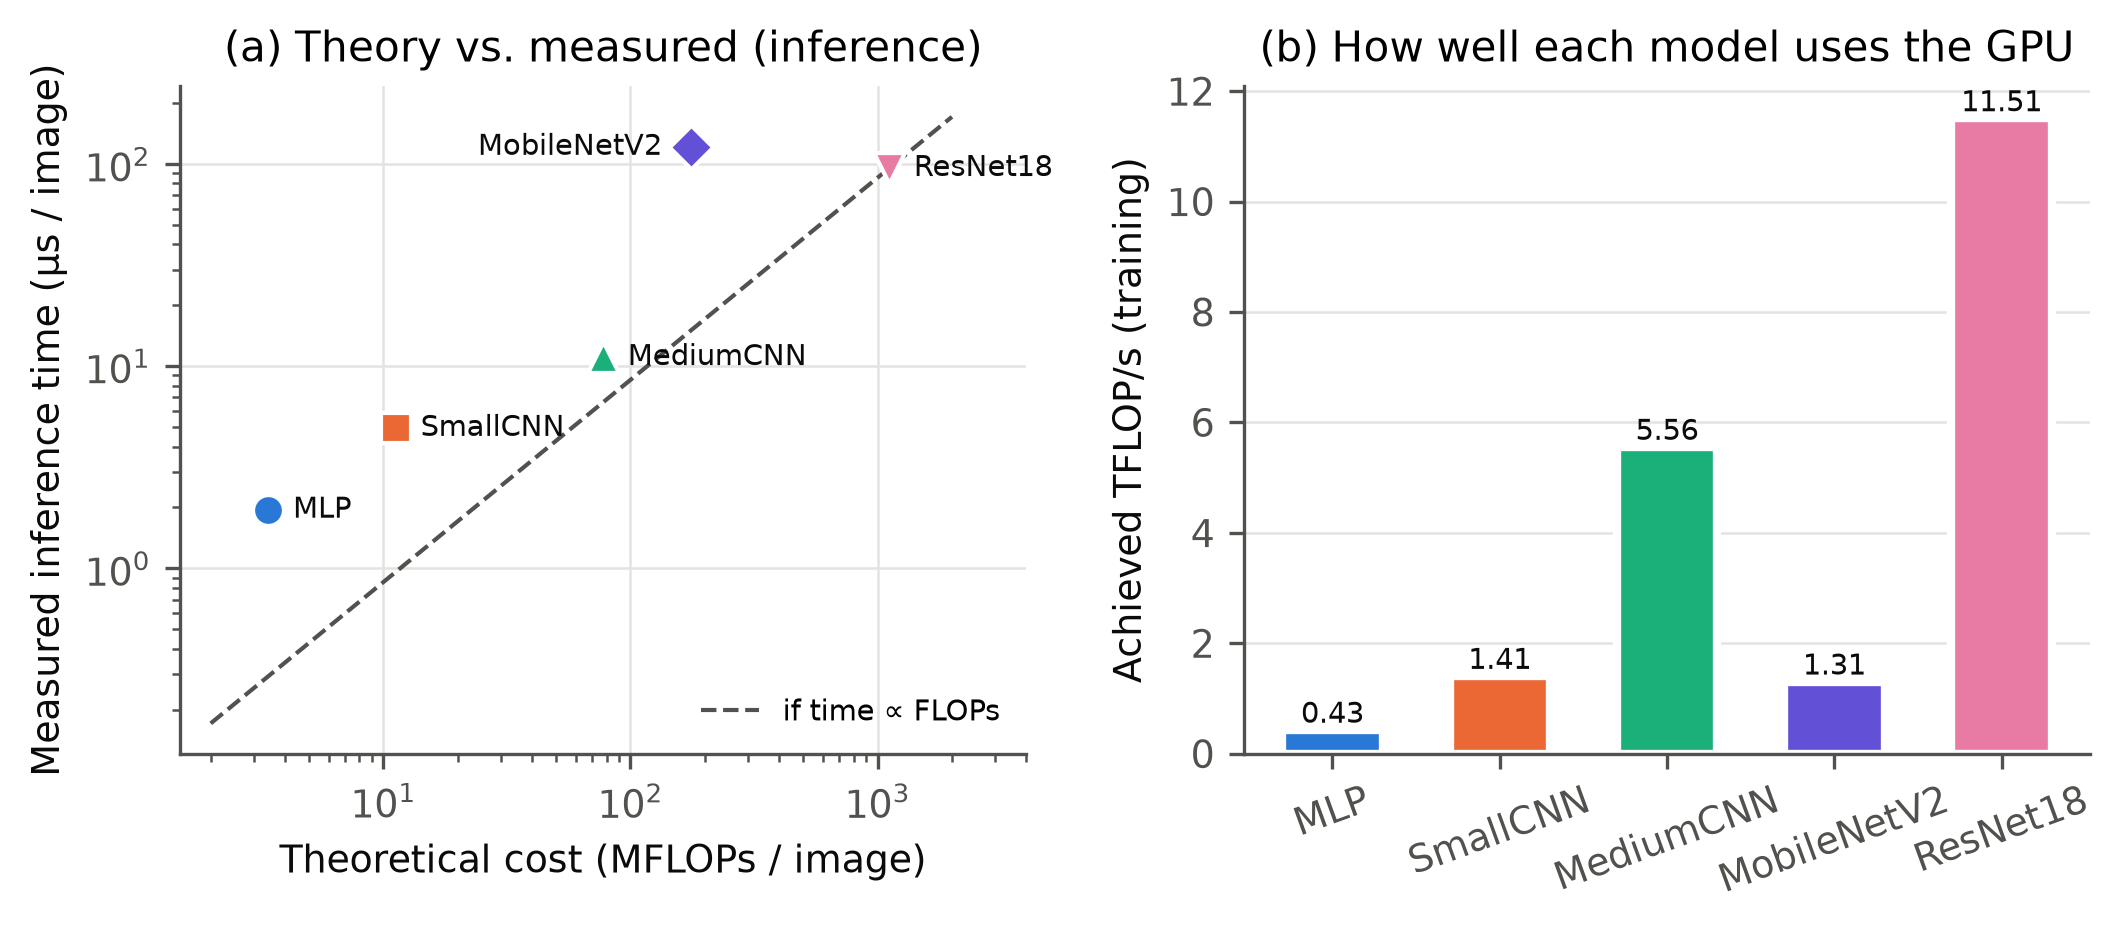
\includegraphics[width=0.64\textwidth]{fig3_theory_vs_measured.png}
\caption{(a) Theoretical cost (FLOPs per image) vs.\ measured inference time per image (batch 512). The dashed line shows the time predicted if time were proportional to FLOPs, anchored at ResNet-18. (b) Achieved training throughput: FLOPs from Eq.~\eqref{eq:work} divided by measured time.}
\label{fig:theory}
\end{figure*}

\subsection{Space}
Parameter count, FLOPs and measured memory give three different rankings (Table~\ref{tab:main}). The MLP has $85\times$ more parameters than SmallCNN but fewer FLOPs and slightly less VRAM. Across the five models the parameter count has a rank correlation of only $\rho=0.6$ with training time, energy and peak training VRAM and $0.7$ with accuracy, whereas FLOPs reach $0.9$ and $1.0$. MobileNetV2 has $5\times$ fewer parameters than ResNet-18 yet needs $2.6\times$ more training VRAM (1227 vs.\ 476\,MB). The reason is the activations stored for backpropagation: its inverted residual blocks expand channels sixfold at high spatial resolution. At inference time, when no activations are kept for a backward pass, the order reverses (354 vs.\ 495\,MB). In a pilot without mixed precision and with batch 512, MobileNetV2 needed 9.2\,GB and overflowed the 8\,GB card, raising its per-image training time $5.1\times$ compared with batch 128. The space complexity of training is thus dominated by activations, not parameters.

\subsection{Energy and the accuracy--energy trade-off}
Average GPU power during training increased with model size, from 34\,W (MLP) to 89\,W (MobileNetV2). The idle draw of the GPU was 24\,W (median over 100 runs). Larger models therefore pay a higher \emph{rate} as well as running longer. For the smallest model only 29\% of the training energy is dynamic, so most of it is idle overhead of an under-used GPU; for the large models the dynamic share is 71--72\%.

Fig.~\ref{fig:pareto} plots accuracy against training energy for all 20 configurations. The Pareto front, where no other configuration is both more accurate and cheaper, is formed almost entirely by MediumCNN at every data size. Only the full-data ResNet-18 extends it. ResNet-18 buys its +3.4 accuracy points over MediumCNN with $7.8\times$ more energy ($6.9\times$ more time). MobileNetV2 is dominated at every data size: from 25\% data upward ResNet-18 is both more accurate \emph{and} cheaper, and at 10\% MediumCNN with 25\% data is. Each model's curve also bends: doubling the data from 50\% to 100\% doubles the energy but adds only 2.4--4.3 accuracy points.

\begin{figure}[t]
\centering
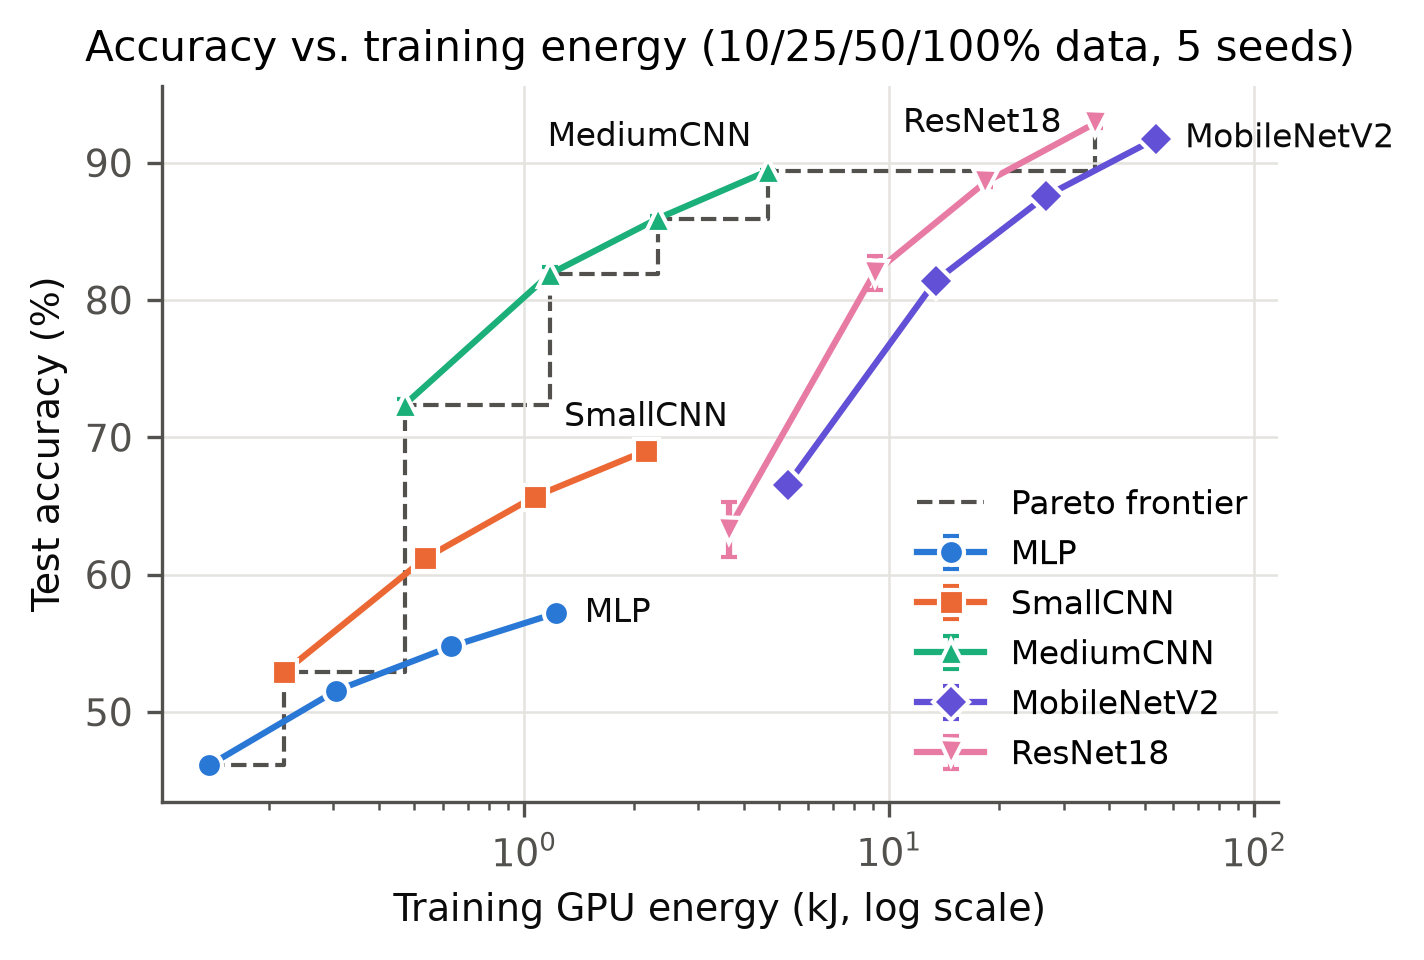
\includegraphics[width=\columnwidth]{fig1_accuracy_vs_energy.png}
\caption{Accuracy vs.\ GPU training energy. Each model has four points (10/25/50/100\% data) with mean $\pm$ std over 5 seeds. The dashed line is the Pareto front.}
\label{fig:pareto}
\end{figure}

\subsection{Inference}
Inference shows the same pattern (Table~\ref{tab:main}). Per image, ResNet-18 consumes 8.0\,mJ and MobileNetV2 10.4\,mJ, compared with 0.96\,mJ for MediumCNN. At batch size 1 the latency of every model is a few milliseconds or less, because GPU launch and transfer overheads dominate. Still, MobileNetV2 (6.6\,ms) is $2\times$ slower than ResNet-18 (3.3\,ms), consistent with its larger number of sequential layers. Throughput at batch 512 spans more than $60\times$, from 8.3k to 516k images/s.


\subsection{Comparison of energy-measurement methods}
We compared three energy-measurement methods with the hardware counter on the full data. Integrating 10\,Hz power samples underestimates the energy by 6--17\%, most for the shortest runs. The NVML power reading is a smoothed value, so short transients are missed. CodeCarbon's GPU figure matches the counter exactly (ratio 1.00), because it reads the same NVML source. It is therefore not an independent check. CodeCarbon's \emph{total} (GPU + CPU + RAM) is 1.6--2.6$\times$ the GPU energy. The host side is thus a large and model-independent share, especially for small models. Its CPU component is a TDP-based estimate on our AMD platform. In total, the 100 runs consumed 908\,kJ (0.25\,kWh) of GPU training energy; according to CodeCarbon, training and inference together emitted about 213\,g CO$_2$.

\subsection{Threats to validity}
\emph{Single platform:} the cross-architecture ranking is specific to a GPU; on a mobile CPU, MobileNetV2's FLOP advantage may materialise~\cite{howard2017mobilenets}. \emph{Fixed recipe:} one shared recipe and 30 epochs ensure fairness but are not optimal for every model; better tuning would raise the accuracies but should not change the cost comparison. \emph{Energy scope:} CPU energy is estimated rather than measured, and very short runs (a few seconds) are subject to counter granularity. \emph{Power management:} laptop power limits depend on the vendor mode; we fixed the mode and logged power, clock and temperature for every run.

% =====================================================================
\section{Conclusion and Future Work}
% =====================================================================
We benchmarked five deep image classifiers on CIFAR-10 across four data sizes and five seeds, measuring performance, time, space and energy together. Asymptotic analysis predicts how cost scales with \emph{data size} very well: time and energy grow linearly and GPU memory stays constant. FLOPs and parameter counts, however, are unreliable predictors of cost \emph{across architectures}. MobileNetV2 has $6.3\times$ fewer FLOPs than ResNet-18 but costs more time, energy and training memory on a GPU, because the achieved throughput varies by a factor of 27 between models. Training memory is governed by activations, not parameters. For an accuracy target around 89\%, a medium-sized CNN is $7.8\times$ more energy-efficient than ResNet-18, and the last few accuracy points are the most expensive.

Practitioners should therefore report measured time and energy on the target hardware next to FLOPs. Future work includes repeating the protocol on CPU and mobile hardware, measuring CPU energy directly on RAPL-capable systems, tuning the recipe per model, and extending the study to larger datasets and transformer-based vision models.

\section*{Code and Data Availability}
All code, raw measurements (one CSV row per run) and figure scripts are available at: \url{https://github.com/akca0/cifar10-beyond-flops}.

\bibliographystyle{IEEEtran}
\bibliography{refs}

\end{document}
